\documentclass[conference]{IEEEtran}

\usepackage{graphicx}
\usepackage{amsmath}
\usepackage{kotex}
\usepackage{url}

% v2 figures live in the figures_v2/ subfolder next to this file.
\graphicspath{{figures_v2/}}

\title{권장과목 기반 학과 군집화와 전문가 검증: 입시 상담 지원을 위한 탐색적 분석}

\author{
  \IEEEauthorblockN{박재우}
  \IEEEauthorblockA{NOVA50301 Term Project --- 포트폴리오 개정판 (v2)}
}

\begin{document}
\maketitle

\begin{abstract}
본 연구는 고등학교 권장과목 정보만으로 대학 학과들을 해석 가능한 방식으로 군집화할 수 있는지, 그리고 그 결과가 현직 입시 전문가의 판단과 부합하는지를 묻는다.
울산 지역 산업 맥락을 반영한 25개 학과를 $25\times89$ 권장과목 binary matrix로 표현하여 inverse document frequency(IDF) 가중 cosine similarity에 hierarchical clustering을 적용하고, 입시 컨설턴트 14명의 card sorting을 $25\times25$ 동시분류 행렬로 집계한 consensus 군집과 Adjusted Rand Index(ARI)로 비교하였다.
거시 구조($k=3$)에서 알고리즘 군집은 전문가 합의와 방향상 일치하나(ARI 점추정 $0.84$, 14명 소패널로 신뢰구간은 넓음), IDF 가중의 이점은 상위 분할이 아니라 세분 구조에서 제한적으로 나타나며 쌍체 부트스트랩 기준 $k=6$에서만 binary 대비 우위가 비교적 견고하다($k=5$는 경향 수준).
실무적으로 권장과목 데이터는 학과 추천의 단독 기준은 아니지만, 전문가 상담에서 놓치기 쉬운 준비과목 기반 대안과 과목 정합성 위험을 탐지하는 보조 신호로 활용될 수 있다.
다만 25개 학과는 목적 표본이고 전문가 패널이 14명으로 작아 일치도의 크기는 단정하기 어려우며, 본 연구는 이를 방향성 위주로 해석한다.
\end{abstract}

% =====================================================================
\section{데이터와 방법}

\subsection{문제와 데이터}

본 프로젝트는 완성된 학과 추천 시스템이 아니라 권장과목 프로파일을 통한 학과 간 준비과목 유사성을 분석하는 탐색적 군집화 연구이다.
분석 대상 25개 학과는 통계적 대표 표본이 아니라 (i) 권장과목 다양성, (ii) 입시 상담 출현 빈도, (iii) 해석 가능성을 고려한 목적 표본이며, 특히 조선해양공학과ㆍ자동차공학과는 울산 주력 산업을 반영한 지역 산업 맥락 기반 공학계열 경계 사례로 포함하였다.
원자료는 학과 과목 선택 가이드이며, 학과별 일반선택ㆍ진로선택ㆍ융합선택 과목을 권장과목으로 제시되면 1, 미언급이면 0으로 코딩하여 $25\times89$ binary matrix를 구성하였다.

\subsection{IDF 가중과 군집화 방법}

학과 vector 간 유사도는 cosine similarity~\cite{manning2008}를 사용하였다.
다만 가이드는 \emph{구체적} 선택과목을 나열하므로, 확률과 통계(21/25 학과)처럼 거의 모든 학과에 공통인 과목이 변별력을 떨어뜨린다.
이를 보정하기 위해 각 과목을 inverse document frequency~\cite{sparck1972}로 가중하였다($w=\ln(N/df)$, 별도 hyperparameter 없음).
군집화는 average linkage hierarchical clustering~\cite{everitt2011}(주 방법)과 k-means~\cite{lloyd1982}를 비교하였다.

\subsection{가중 기준의 근거}

가중치를 임의로 정하지 않기 위해, 본 연구는 정보검색의 표준 가중인 IDF를 채택하였다.
IDF는 (i) 손으로 정하는 모수가 없이 과목별 가중이 출현 빈도로 결정되고, (ii) 흔한 과목을 자동으로 저가중하여 ``공통 과목이 변별력을 떨어뜨린다''는 문제에 직접 대응한다.
실제로 선택과목 유형별 평균 IDF는 일반선택 $0.99$, 진로선택 $1.29$, 융합선택 $1.85$로 더 특수한 과목일수록 높은 가중을 받는다 --- 이는 ``진로선택이 가장 변별적''이라는 직관과 어긋나, 임의의 유형별 가중(예: 진로$=3$)이 오히려 데이터와 반대 방향임을 보여준다.
따라서 유형 단위의 임의 가중 대신 과목 단위 IDF를 사용하였다.
나아가 가중 강도를 $w=\mathrm{idf}^{\alpha}$의 단일 조절 모수로 $\alpha\!\in\![0,2]$ 범위에서 흔든 민감도 분석에서($\alpha=0$ 무가중, $\alpha=1$ 표준 IDF) $\alpha=1$은 군집 구조가 일정하게 유지되는 안정 구간에 위치하여, 특정 가중을 골라 끼워맞춘 결과가 아님을 확인하였다.
가중 기준은 card sorting과 독립적으로 데이터 내부 기준만으로 결정하여, 전문가 검증의 외부성을 훼손하지 않았다.
이러한 변별력 차이는 과목 수준에서 직접 드러난다(Table~\ref{tab:discriminative}): 특정 계열 군집에만 등장하는 과목은 그 군집을 변별하는 반면, 확률과 통계(21/25 학과)와 같은 공통 과목은 변별력이 거의 없다.

\begin{table}[!ht]
\centering
\caption{변별력 대조 --- 특정 계열 군집에만 등장하는 과목은 그 군집을 변별하나, 공통 과목은 변별력이 거의 없다.}
\label{tab:discriminative}
\begin{tabular}{lccl}
\hline
과목 & df & IDF & 권장 학과 군집 \\
\hline
\multicolumn{4}{l}{\textit{군집 변별 과목 (특정 계열 군집에만 등장)}} \\
창의공학 설계 & 6 & 1.43 & 공학 6개 \\
경제 수학 & 3 & 2.12 & 경영학·경제학·응용통계학 \\
보건 & 2 & 2.53 & 간호학·약학 \\
언어생활 탐구 & 2 & 2.53 & 국어국문학·사학 \\
\hline
\multicolumn{4}{l}{\textit{저변별 (공통 과목, 변별 거의 없음)}} \\
확률과 통계 & 21 & 0.17 & 공통(21개 학과) \\
대수 & 17 & 0.39 & 공통(17개 학과) \\
정보 & 16 & 0.45 & 공통(16개 학과) \\
기하 & 15 & 0.51 & 공통(15개 학과) \\
미적분Ⅰ & 15 & 0.51 & 공통(15개 학과) \\
\hline
\end{tabular}
\end{table}

\subsection{$k$의 역할}

본 연구에서 $k$ 값은 단일 최적값을 찾기 위한 목적이 아니라, 군집 구조의 해상도별 변화를 관찰하기 위해 사용하였다.
$k=3$은 권장과목 기반 거시 구조를 확인하기 위한 기준이며, $k=4$는 전문가 consensus clustering과의 주 비교 단위로 사용하였다.
$k=5$와 $k=6$은 세분 구조에서 IDF 가중의 효과가 나타나는지를 확인하기 위한 민감도 분석이며, $k=7$은 binary 기준에서 의약-보건 군집이 분리되는 시점을 설명하기 위한 보조 cut으로 사용하였다.

% =====================================================================
\section{내부 군집 분석}

표준 IDF 가중($\alpha=1$)으로 $k=4$ hierarchical 군집을 보면 (a) STEM-보건 17개 대군집, (b) 국어국문ㆍ디자인, (c) 경영ㆍ경제, (d) 심리ㆍ사회ㆍ미디어ㆍ사학으로 나뉜다(Fig.~\ref{fig:idf_dendrogram}).
즉 상위 수준 구조는 무가중 binary와 마찬가지로 \emph{STEM-보건 대군집}이 지배하며, 내부 지표상 IDF가 binary를 능가하지는 않는다(silhouette $0.24$ vs $0.33$, 계열 ARI $0.27$ vs $0.32$).
IDF 가중의 효과는 상위 수준 분할이 아니라 과목 변별(Table~\ref{tab:discriminative})과 아래의 세부 구조에서 나타난다.

\begin{figure*}[t]
  \centering
  
\includegraphics[width=0.86\linewidth]{idf_dendrogram.png}
  \caption{IDF 가중 dendrogram(average linkage, cosine distance), $k=4$ 군집명 표기. 의약-보건(의예ㆍ약학ㆍ간호)이 뚜렷한 하위 가지를 이루며($k=5$에서 코어로부터 분리), 자동차공학과는 기계공학과와 가장 작은 거리에서 결합한다.}
  \label{fig:idf_dendrogram}
\end{figure*}

STEM-보건 17개 대군집을 코어 내에서 재가중하여 하위 군집화하면(Fig.~\ref{fig:subcluster}, complete linkage, $k=3$), (i) 의약-보건(의예ㆍ약학ㆍ간호), (ii) 정량ㆍ응용(산업ㆍ수학ㆍ응용통계ㆍ식품영양), (iii) 공학-화학 10개(건축ㆍ기계ㆍ화학ㆍ신소재ㆍ조선해양ㆍ생명ㆍ화학공학ㆍ전기전자ㆍ컴퓨터ㆍ자동차)로 분리된다.
의약-보건은 average linkage 전체 트리에서 IDF는 $k=5$, binary는 $k=7$에서 코어로부터 분리되어, 가중이 의약-보건 신호를 상대적으로 더 일찍 드러낸다.

\begin{figure}[!ht]
  \centering
  
\includegraphics[width=\linewidth]{idf_core_subdendrogram.png}
  \caption{STEM-보건 17개 대군집의 하위 군집화(코어 내 IDF 재가중, complete linkage). 세 하위 가지로 나뉘나, 특징(과목) 재표집 안정성은 세 가지 모두 중간 수준이다(Table~\ref{tab:stability}).}
  \label{fig:subcluster}
\end{figure}

\subsection{코어 하위 군집 안정성}

위 하위 군집이 특정 과목 집합에 의존하지 않는지를 검증하기 위해, 코어에 등장하는 과목 특징을 복원추출로 $B=1000$회 재표집(seed 고정)하여 매번 local IDF를 재계산하고 하위 군집화를 반복하였다(Hennig clusterboot 방식, cluster별 최대 Jaccard~\cite{hennig2007,efron1979}).
세 하위 군집의 안정성은 의약-보건 $0.56\,[0.25,1.00]$, 정량ㆍ응용 $0.56\,[0.23,1.00]$, 공학-화학 $0.58\,[0.31,1.00]$로 \emph{모두 중간 수준}이며 서로 큰 차이가 없다(Table~\ref{tab:stability}, Panel A).
즉 코어 내부의 세부 분할은 어느 가지도 특징 재표집에 견고하지 않으며, 의약-보건 역시 다른 가지보다 특별히 안정적이지는 않다.

\subsection{방법 간 강건성}

군집화 방법 의존성을 점검하기 위해 hierarchical(주 방법)과 k-means를 동일한 IDF 벡터에서 비교하였다.
두 방법은 거시 구조에서 어느 정도 일치하나($k=3$ ARI $0.46$, $k=5$ $0.53$), $k=4$ 경계에서는 갈린다(ARI $0.37$).
즉 거시 구조는 비교적 방법에 강건하나 세부 경계는 군집화 방법과 가중 모두에 민감하며, 이는 아래 내부ㆍ외부 비교 결과와 일관된다.

% =====================================================================
\section{전문가 검증}

내부 평가 지표는 군집의 기하학적 특성만 측정하므로, 본 연구는 외부 기준으로 현직 입시 컨설턴트 14명의 card sorting~\cite{spencer2009}을 활용한다.
과제는 open card sort이며, 25개 학과 카드를 ``권장과목 관점에서 비슷한 학과끼리'' 그룹 수 제한 없이 자유롭게 분류한다(사전 $k$ 미강제, 독립 판단 보장).
14명 분류를 $25\times25$ 동시분류(co-occurrence) 행렬로 집계하고, $1-$동시분류율을 거리로 하는 average linkage로 consensus clustering을 도출하였다.

Consensus 군집($k=4$)은 (i) 사회ㆍ인문 7개(국어ㆍ심리ㆍ경영ㆍ사회ㆍ경제ㆍ미디어ㆍ사학), (ii) 의약-보건(의예ㆍ약학ㆍ간호), (iii) 건축ㆍ디자인, (iv) 공학-자연 13개로 나타났다(Fig.~\ref{fig:heatmap}).
consensus 군집의 견고성은 14명을 복원추출로 $B=1000$회 재표집(seed 고정)하여 매번 동시분류 행렬과 consensus clustering을 재계산하고 cluster별 최대 Jaccard를 집계해 검증하였다(Table~\ref{tab:stability}, Panel B).
전문가 관점의 인사이트는 다음과 같다.
첫째, 의예-약학은 전문가 전원이 함께 묶었으나(동시분류 $1.0$) 간호는 더 느슨하게 결합하여(의예-간호ㆍ약학-간호 $0.57$), 의약-보건 3개 군집의 rater 재표집 안정성은 $0.56\,[0.33,1.00]$로 중간 수준에 그쳤고, 화학ㆍ생명ㆍ식품영양을 포함하는 광의의 바이오-보건 경계는 전문가 사이에서도 갈렸다.
둘째, 건축ㆍ디자인은 최대 동시분류율이 $0.14$에 불과하고 consensus 안정성도 $0.70\,[0.29,1.00]$로 하한이 낮아, 어떤 군집에도 합의되지 못하는 가장 모호한 경계 학과로 확인되었다(Fig.~\ref{fig:ambiguity}).
셋째, 가장 견고하게 합의된 군집은 사회ㆍ인문 7개로($0.88\,[0.70,1.00]$), 권장과목 거시 구조가 인문ㆍ사회 영역에서 특히 안정적이다.
넷째, 울산 경계 사례인 자동차ㆍ조선해양공학과는 공학 대군집에 명확히 합의되어 모호하지 않았다.

\begin{figure}[!ht]
  \centering
  
\includegraphics[width=\linewidth]{cardsort_cooccurrence_heatmap.png}
  \caption{전문가 동시분류 행렬(14명, consensus 군집 순서, 군집 경계선 강조). 의약-보건ㆍ사회/인문 블록이 뚜렷하며, 건축ㆍ디자인은 어떤 학과와도 동시분류율이 낮다.}
  \label{fig:heatmap}
\end{figure}

\begin{figure}[!ht]
  \centering
  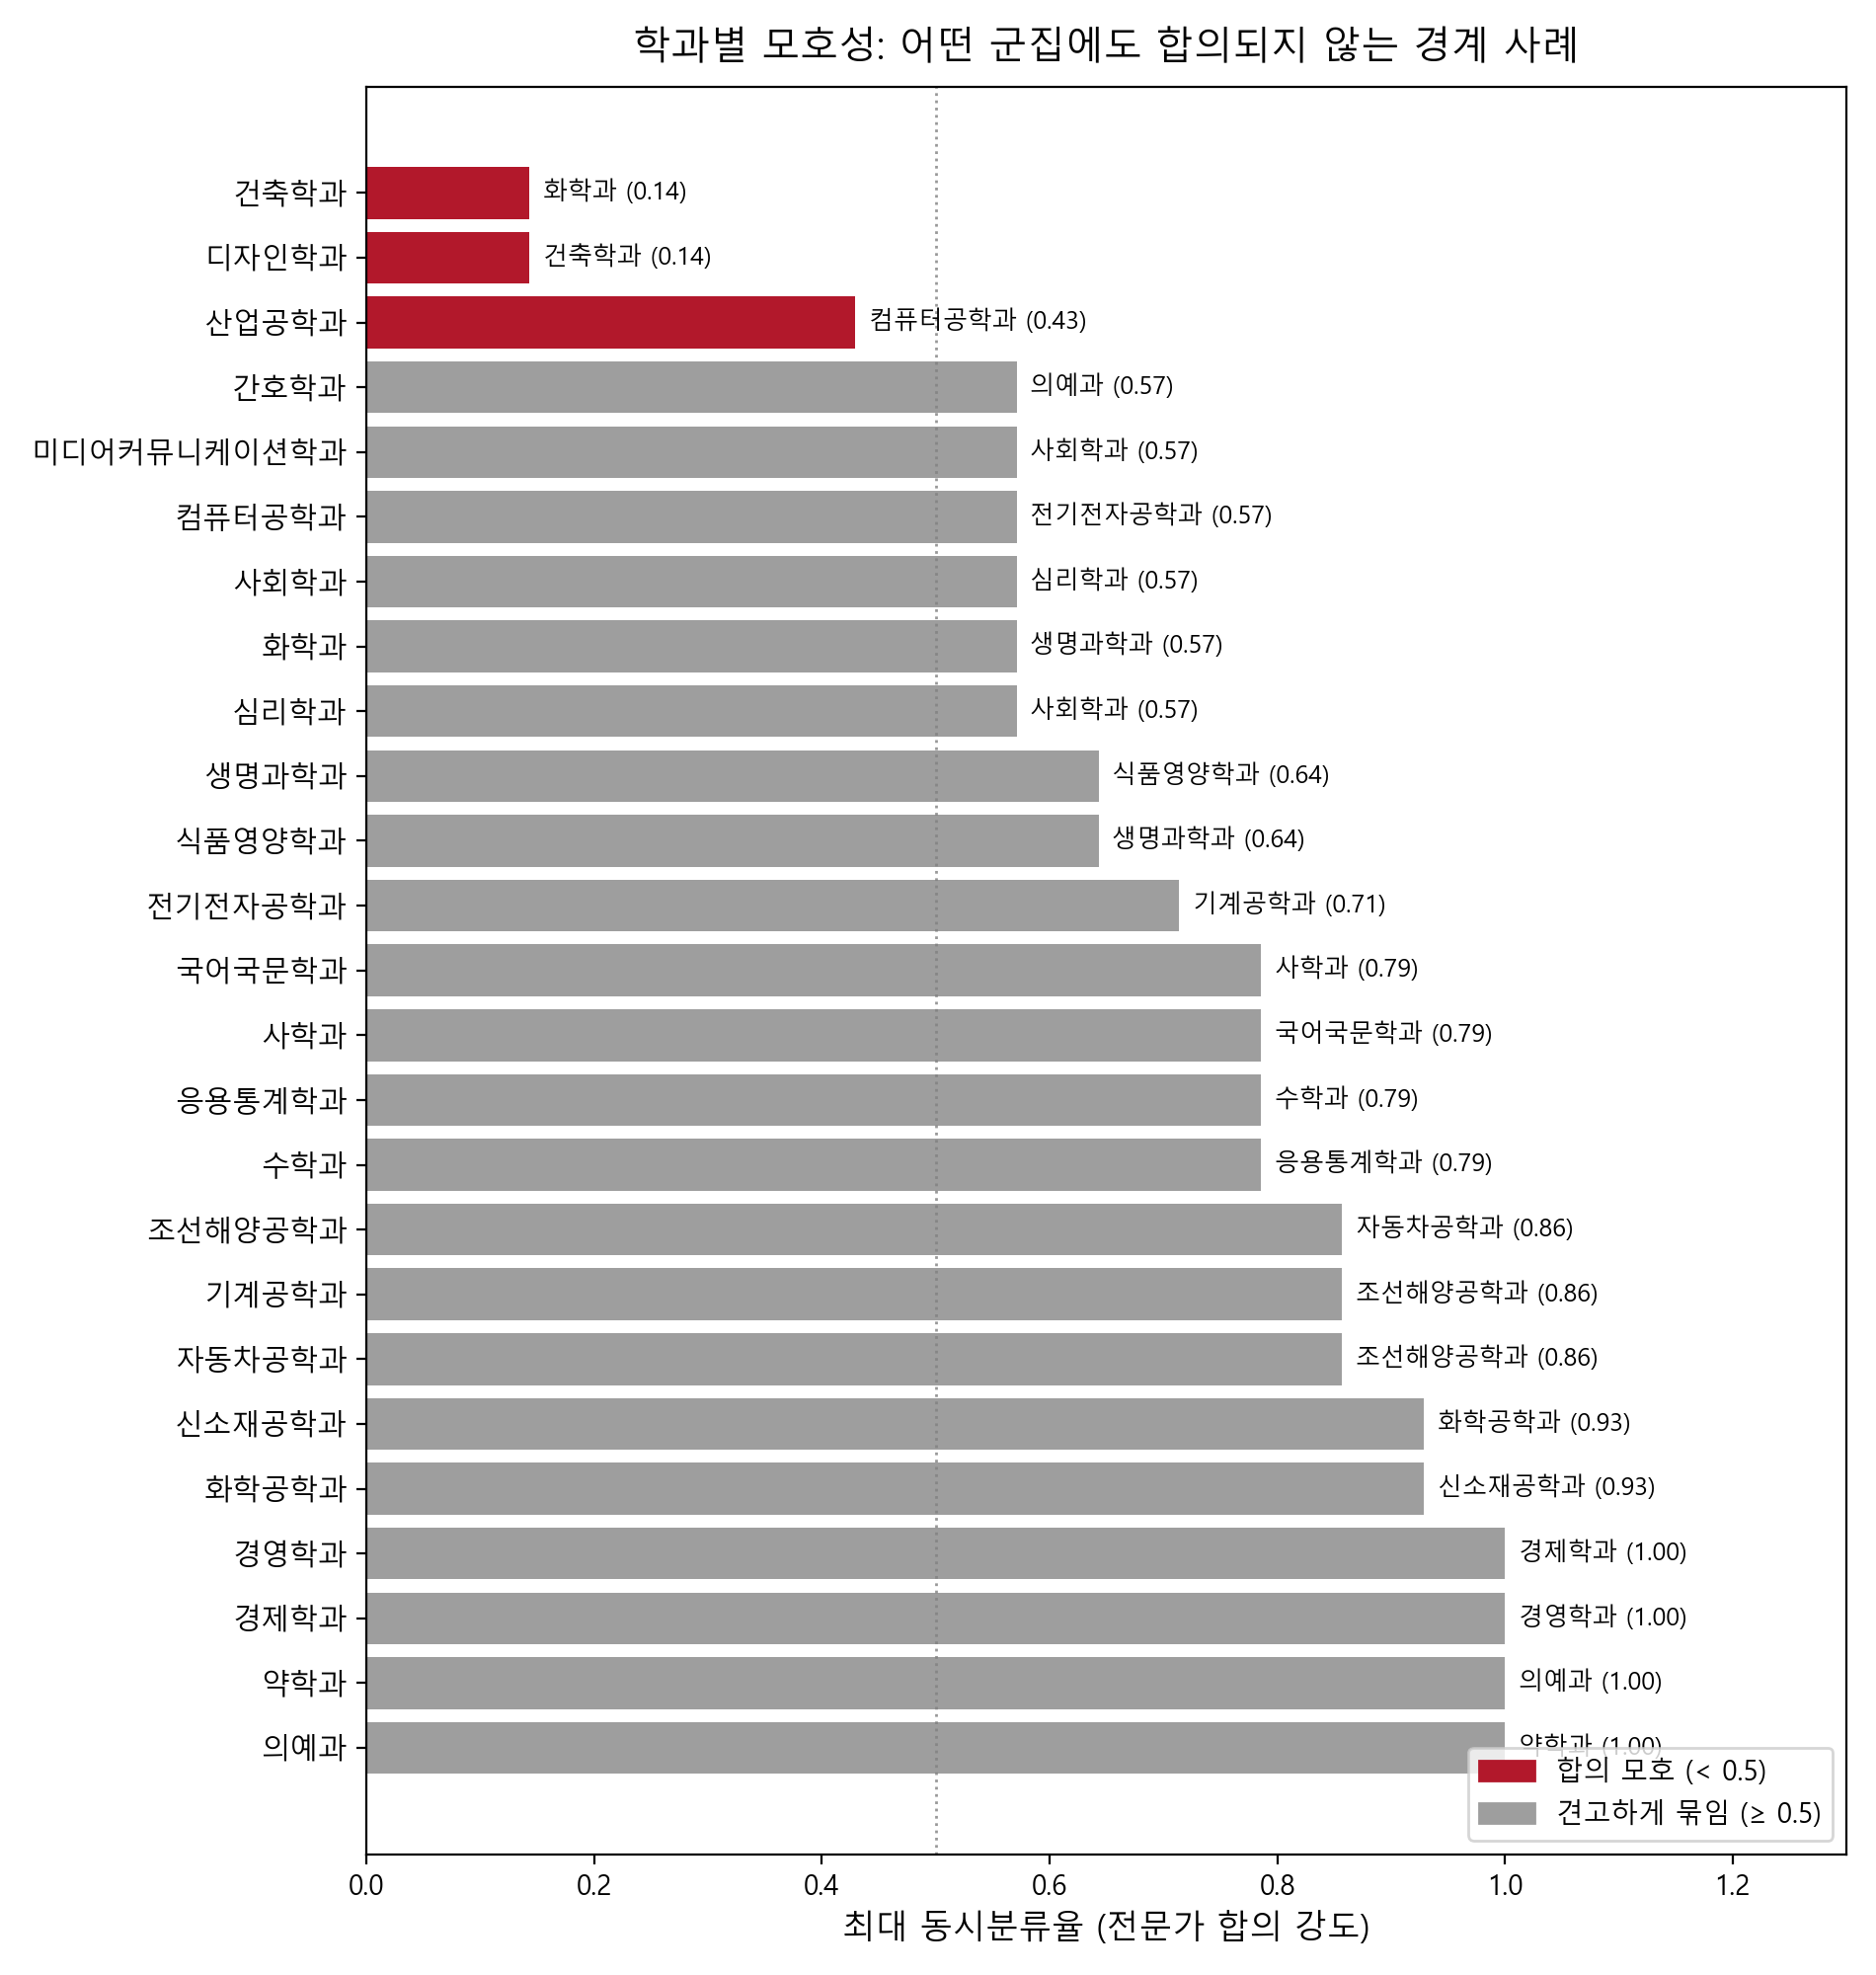
\includegraphics[width=\linewidth]{cardsort_department_ambiguity_bars.png}
  \caption{학과별 최대 동시분류율(전문가 합의 강도) 오름차순. $0.5$ 미만(건축ㆍ디자인ㆍ산업공학)은 어떤 군집에도 합의되지 않는 경계 학과이며, 막대 끝 라벨은 가장 가까운 학과와 그 값이다.}
  \label{fig:ambiguity}
\end{figure}

% =====================================================================
\section{내부 vs 전문가 비교}

내부 군집과 외부(전문가) 합의의 일치도는 $k$에 따라 달라지며, 14명 소패널을 반영해 rater 부트스트랩 $95\%$ CI를 함께 보고한다($B=1000$, seed 고정, Fig.~\ref{fig:agree}).
거시 구조($k=3$)에서 점추정은 IDF와 binary 모두 ARI~\cite{hubert1985} $0.84$이나 CI가 $[0.04,0.95]$로 매우 넓어, 거시 일치의 \emph{방향}은 일관되나 그 크기는 표본 한계로 불확실하다.
상위 수준 $k=4$에서는 두 방법 모두 STEM-보건을 분리하지 못해 일치도가 낮고 CI도 겹친다(IDF $0.52\,[0.09,0.62]$, binary $0.59\,[0.17,0.68]$).
$k=6$에서 IDF 점추정 ARI($0.35$)는 binary($0.11$)보다 높다.
두 방법의 개별 신뢰구간은 일부 겹치지만, 동일 부트스트랩 표본에서 계산한 쌍체 차이($\mathrm{ARI}_{\mathrm{IDF}}-\mathrm{ARI}_{\mathrm{binary}}$)의 $95\%$ 신뢰구간은 $[0.06,0.32]$로 0을 포함하지 않아, 세분 구조에서 IDF의 우위는 비교적 견고하다(1000회 중 $99.4\%$에서 양수).
반면 $k=5$에서는 같은 쌍체 차이의 신뢰구간이 $[-0.08,0.20]$로 0을 포함하므로, IDF가 유리한 경향은 있으나 통계적으로 확정하기는 어렵다.
한편 상위 분할인 $k=4$에서는 쌍체 차이가 $[-0.08,-0.04]$로 binary가 근소하게 견고한 우위를 보이는데, 이는 STEM-보건 대군집이 지배하는 상위 구조에서는 IDF 가중의 효과가 제한적이며 그 이점이 세분 단위($k\!\ge\!6$)에서 비로소 나타난다는 본 연구의 해석과 일관된다.
즉 권장과목은 전문가의 \emph{거시} 판단과 방향상 일치하나 표본 한계로 크기는 불확실하고, IDF 가중의 비교적 견고한 이점은 세분 단위, 특히 $k=6$에서 드러난다.

\begin{figure}[!ht]
  \centering
  
\includegraphics[width=\linewidth]{cardsort_agreement_bars.png}
  \caption{알고리즘 군집 vs 전문가 합의의 ARI(오차막대: rater 부트스트랩 $95\%$ CI, $B=1000$). $k=3$ 점추정은 양쪽 $0.84$이나 소패널로 CI가 넓고, $k=6$에서 IDF가 binary보다 높으며 쌍체 차이의 $95\%$ 신뢰구간이 0을 제외한다($k=5$는 0 포함).}
  \label{fig:agree}
\end{figure}

\begin{table}[!ht]
\centering
\caption{군집 안정성(부트스트랩 $B=1000$, Jaccard 평균 $[95\%$ CI$]$). Panel A는 코어 하위 군집의 특징(과목) 재표집, Panel B는 전문가 consensus($k=4$)의 rater 재표집.}
\label{tab:stability}
\begin{tabular}{lc}
\hline
군집 & Jaccard $[95\%$ CI$]$ \\
\hline
\multicolumn{2}{l}{\emph{Panel A. 코어 하위 군집 (특징 부트스트랩)}} \\
의약-보건(의예ㆍ약학ㆍ간호) & 0.56 [0.25, 1.00] \\
정량ㆍ응용(산업ㆍ수학ㆍ응용통계ㆍ식품영양) & 0.56 [0.23, 1.00] \\
공학-화학 10개 & 0.58 [0.31, 1.00] \\
\hline
\multicolumn{2}{l}{\emph{Panel B. 전문가 consensus $k=4$ (rater bootstrap)}} \\
사회ㆍ인문 7개 & 0.88 [0.70, 1.00] \\
공학-자연 13개 & 0.66 [0.36, 0.93] \\
건축ㆍ디자인 & 0.70 [0.29, 1.00] \\
의약-보건(의예ㆍ약학ㆍ간호) & 0.56 [0.33, 1.00] \\
\hline
\end{tabular}
\end{table}

cut에 무관한 쌍 수준 지표에서는 동시분류율과 IDF cosine similarity가 양의 상관을 보여($r=0.68$, Fig.~\ref{fig:scatter}), 내부ㆍ외부가 전반적으로 정렬됨을 확인한다.
각 쌍의 두 값을 표준화한 격차로 불일치를 두 유형으로 구분하였다(대표 쌍은 Table~\ref{tab:disagree}).
\textbf{Type 1(내부 O, 외부 X)}: 준비기반은 유사하나 전문가가 분리하는 쌍이다.
신소재공학-생명과학(IDF $0.66$, 동시분류 $0.14$), 화학-자동차공학($0.51$, $0.00$) 등은 수학ㆍ과학 공통 준비기반을 공유하지만 진로 목적지가 달라 상담에서 분리된다.
\textbf{Type 2(내부 X, 외부 O)}: 권장과목은 갈리나 전문가가 묶는 쌍이다.
대표 사례인 조선해양공학-자동차공학(IDF $0.31$, 동시분류 $0.86$)은 ``울산 산업공학''으로 함께 추천되지만, 권장과목은 조선해양(화학ㆍ재료)과 자동차(기계ㆍ전자ㆍ소프트웨어)로 분기한다.
국어국문-사학($0.11$, $0.79$), 생명과학-식품영양($0.32$, $0.64$)도 같은 유형이다.
대부분의 불일치는 알고리즘이 STEM-보건을 하나의 큰 코어로 묶어 발생하는 내부O-외부X 유형이며, 이는 하위 군집화와 더 세분한 $k$에서 완화된다.

\begin{table}[!ht]
\centering
\caption{내부-외부 불일치 대표 학과 쌍. IDF cos는 내부 유사도, 동시분류는 전문가 외부 합의.}
\label{tab:disagree}
\begin{tabular}{llcc}
\hline
유형 & 학과 쌍 & IDF cos & 동시분류 \\
\hline
Type 1 & 신소재공학-생명과학 & 0.66 & 0.14 \\
Type 1 & 화학-조선해양공학 & 0.53 & 0.00 \\
Type 1 & 화학-자동차공학 & 0.51 & 0.00 \\
Type 2 & 조선해양공학-자동차공학 & 0.31 & 0.86 \\
Type 2 & 국어국문-사학 & 0.11 & 0.79 \\
Type 2 & 생명과학-식품영양 & 0.32 & 0.64 \\
\hline
\end{tabular}
\end{table}

\begin{figure}[!ht]
  \centering
  
\includegraphics[width=\linewidth]{cardsort_cooccur_vs_idf_scatter.png}
  \caption{학과 쌍(n=300): IDF cosine similarity(내부) vs 전문가 동시분류율(외부). 대각선에서 벗어난 쌍이 불일치 사례이며, Table~\ref{tab:disagree}의 대표 쌍을 표시하였다.}
  \label{fig:scatter}
\end{figure}

% =====================================================================
\section{실무 적용}

세 단계(내부 군집ㆍ전문가 합의ㆍ둘의 비교)의 결과는 알고리즘과 전문가의 일치/불일치 사분면으로 정리되어 입시 상담 워크플로우에 결합될 수 있다(Table~\ref{tab:quadrant}).
첫째, 알고리즘과 전문가가 함께 묶는 군집(예: 의약-보건)은 \emph{신뢰 가능한 추천 단위}로 사용한다.
둘째, \textbf{Type 1}(알고리즘 O / 전문가 X) 쌍은 ``공통 준비기반 대안'' 추천에 활용한다 --- 한 학과를 준비한 학생은 다른 학과의 과목 토대를 이미 상당 부분 갖추고 있으므로, 상담이 간과하기 쉬운 교차 계열 선택지를 알고리즘이 자동으로 제시할 수 있다.
셋째, \textbf{Type 2}(알고리즘 X / 전문가 O) 쌍은 \emph{준비 정합성 경고}로 활용한다 --- 컨설턴트가 함께 추천하더라도 권장과목이 분기하면, 학생의 과목 이수가 목표 학과와 어긋날 위험을 사전에 표시한다(예: 자동차 준비 학생의 조선해양 추천 시 재료ㆍ화학 보강 안내).
넷째, 양쪽 모두에서 관련성이 낮은 쌍은 추천 후순위로 둔다.
이러한 방식은 울산 고교 과목로드맵 DB와 연계하여, 학생의 실제 이수 과목과 학과별 권장과목 프로파일을 대조하는 의사결정 보조 도구로 확장 가능하다.

\begin{table}[!ht]
\centering
\footnotesize
\caption{알고리즘 군집과 전문가 합의의 일치/불일치 사분면과 상담 활용.}
\label{tab:quadrant}
\begin{tabular}{p{0.26\linewidth}p{0.33\linewidth}p{0.29\linewidth}}
\hline
유형 & 의미 & 상담 활용 \\
\hline
알고리즘 O · 전문가 O & 안정 추천군 & 우선 추천 단위 \\
Type 1 (알고리즘 O · 전문가 X) & 전문가가 놓칠 수 있는 준비기반 유사 학과 & 교차 계열 대안 제시 \\
Type 2 (알고리즘 X · 전문가 O) & 전문가 직관상 함께 추천되나 권장과목은 분기 & 과목 정합성 경고, 보강 과목 안내 \\
알고리즘 X · 전문가 X & 준비과목ㆍ직관 모두 낮은 관련성 & 추천 후순위 \\
\hline
\end{tabular}
\end{table}

% =====================================================================
\section{향후 과제: 전 학과로의 일반화}

본 연구의 핵심 후속 질문은 \emph{25개 학과에서 확인된 권장과목 유사성 구조를 전(全) 학과로 확장할 수 있는가}이다.
방법론적으로 권장과목 vector는 권장과목 프로파일이 존재하는 임의의 학과에 동일하게 정의되므로, 전 학과에 대해 동일한 IDF 가중 vector를 구성하고 본 연구에서 거시 구조가 전문가 합의와 방향상 일치함을 확인한 군집 공간에 투영(projection)하는 접근이 가능하다.
다만 (i) 학과 수가 늘면 권장과목 해상도의 한계(공학-자연 대군집 문제)가 심화될 수 있고, (ii) 25개 표본에서 학습된 IDF 가중과 군집 경계가 전 학과 분포에서 그대로 유지된다는 보장이 없으며, (iii) 전문가 검증을 전 학과로 확대하는 비용이 크다는 과제가 있다.
따라서 25개 학과를 \emph{앵커(anchor)}로 삼아 신규 학과를 가장 가까운 앵커 군집에 배정하고, 경계 사례에 한해 전문가 검증을 선택적으로 수행하는 준지도(semi-supervised) 확장이 현실적 경로로 보인다.

% =====================================================================
\section{한계 및 후속 연구}

본 연구의 한계는 다음 네 가지로 정리된다.
\begin{enumerate}
\item \textbf{표본 한계}: 25개 학과는 목적 표본이므로 전체 학과로의 일반화에 한계가 있다.
\item \textbf{권장과목 해상도 한계}: 수학ㆍ과학 공통 과목이 많아 상위 수준 $k=4$에서 STEM-보건 17개가 하나의 대군집을 이루며, 세부 전공 차이를 충분히 반영하지 못한다. IDF 가중은 이 상위 분할 자체를 바꾸지 못하고, 그 이점은 과목 변별과 세분 구조($k=6$)에 국한된다.
\item \textbf{전문가 패널 한계}: 입시 컨설턴트 14명의 소패널이므로 rater 부트스트랩에서 합의 일치도 ARI의 CI가 넓게 나타나며(Fig.~\ref{fig:agree}), 일치도의 \emph{크기}는 단정하기 어렵다(1명은 과도 세분으로 민감도 분석 처리). 본 연구는 일치도를 방향성 위주로 해석한다.
\item \textbf{성과 검증 한계}: 실제 입결ㆍ합격 가능성ㆍ학생 선택 결과와 연결하지 못하였다.
\end{enumerate}

코어 하위 군집의 안정성은 본 보고서에서 특징 부트스트랩으로 정량화하여 마무리하였다(Table~\ref{tab:stability}). 남은 후속 연구는 다음 두 가지이다.
\begin{enumerate}
\item 입결 feasibility를 결합한 Type 2 ``준비 정합성 위험''의 정량화.
\item 전 학과 일반화를 위한 anchor 기반 준지도 확장.
\end{enumerate}
두 과제 모두 추가 데이터(입결)와 전문가 검증 비용을 요한다.

% =====================================================================
% TODO: 제출 전 각 참고문헌의 권/호/페이지를 원문과 대조하여 최종 확인할 것
%       (특히 Spencer 2009 판차, Hennig 2007 권/호/페이지).
\begin{thebibliography}{9}
\bibitem{sparck1972} K. Spärck Jones, ``A statistical interpretation of term specificity and its application in retrieval,'' \emph{Journal of Documentation}, vol. 28, no. 1, pp. 11--21, 1972.
\bibitem{manning2008} C. D. Manning, P. Raghavan, and H. Schütze, \emph{Introduction to Information Retrieval}. Cambridge, U.K.: Cambridge Univ. Press, 2008.
\bibitem{everitt2011} B. S. Everitt, S. Landau, M. Leese, and D. Stahl, \emph{Cluster Analysis}, 5th ed. Chichester, U.K.: Wiley, 2011.
\bibitem{lloyd1982} S. P. Lloyd, ``Least squares quantization in PCM,'' \emph{IEEE Trans. Inf. Theory}, vol. 28, no. 2, pp. 129--137, 1982.
\bibitem{hubert1985} L. Hubert and P. Arabie, ``Comparing partitions,'' \emph{Journal of Classification}, vol. 2, no. 1, pp. 193--218, 1985.
\bibitem{spencer2009} D. Spencer, \emph{Card Sorting: Designing Usable Categories}. Brooklyn, NY, USA: Rosenfeld Media, 2009.
\bibitem{hennig2007} C. Hennig, ``Cluster-wise assessment of cluster stability,'' \emph{Computational Statistics \& Data Analysis}, vol. 52, no. 1, pp. 258--271, 2007.
\bibitem{efron1979} B. Efron, ``Bootstrap methods: Another look at the jackknife,'' \emph{The Annals of Statistics}, vol. 7, no. 1, pp. 1--26, 1979.
\end{thebibliography}

\end{document}
